\startchapter{Experiments, Evaluation and Comparisons}
\label{chapter:eval}
This chapter presents results of the simulations and experiments done to evaluate the proposed solutions in both single and multi-hop transmission chapters. In order to gain confidence in the final results and eliminate unwanted errors, all parameters are measured with extensive iterations and averaging. Wherever possible, comparisons have been made with other widely used algorithms to better illustrate the contribution of this thesis. 

\section{RSS-Based Grouping Strategy}

%The simulations used in this section are all done by MATLAB and NS-2\cite{breslau2000advances}.

%The results in this section are produced 
The performance of different grouping schemes is evaluated using MATLAB and NS-2\cite{breslau2000advances}. MATLAB is used for numerical calculations and NS-2 is used for throughput simulations. The network coverage is assumed to be a circle with radius $1$ km which is the case in sub 1GHz network having the access point at the center. As mentioned in Section \ref{systemmodel}, nodes are uniformly placed in the coverage area with their number following a Poisson distribution with density 0.0019 node per square meter which results in 6000 nodes in the network on average. The number of groups, M, was set in the range of 8 to 512. For each setting, the experiments were repeated 20 times, and the average was taken. 

%For each scheme the grouping is done 20 times and at each iteration an average is taken on all groups.

%We have first used our two predefined metrics to compare grouping schemes. We also calculate those metrics using a K-means clustering algorithm. 

If the AP the knows location information of all the nodes, in a pure centralized solution where AP decides the group for each node, the k-means algorithm can be used to achieve near-optimal groupings. So we can use the performance with k-means grouping as a benchmark to see how well our RSS-based distributed grouping algorithm is working compared with the centralized benchmark.

In Fig. \ref{fig:meansum}, the average distance between nodes in a group for the proposed scheme is always smaller than with the random grouping scheme and close to the k-means clustering algorithm. It is also obvious that a larger number of groups have a smaller average distance between nodes for all algorithms. 

In Fig. \ref{fig:variance}, we can see that the standard deviation of the number of nodes in different groups is the cost that the RSS-based grouping algorithm pays for the advantage of distributed solution. Groups with a large number of users will suffer from high collision probability and groups with a very small number of users may not fully utilize their RAW. It is shown later using NS-2 simulations, that despite having some dense groups, the RSS-based grouping algorithm has a better performance than random groupings. This is because the hidden node problem is a more severe problem than uneven groups. A few hidden terminals can dramatically decrease the performance of the whole network. Having more nodes that are all in the sensing range increases the competition but has a less destructive effect on the throughput than that due to hidden terminal.



\begin{figure}
  \centering
  \subfloat[][Average $D_m$ over all groups]{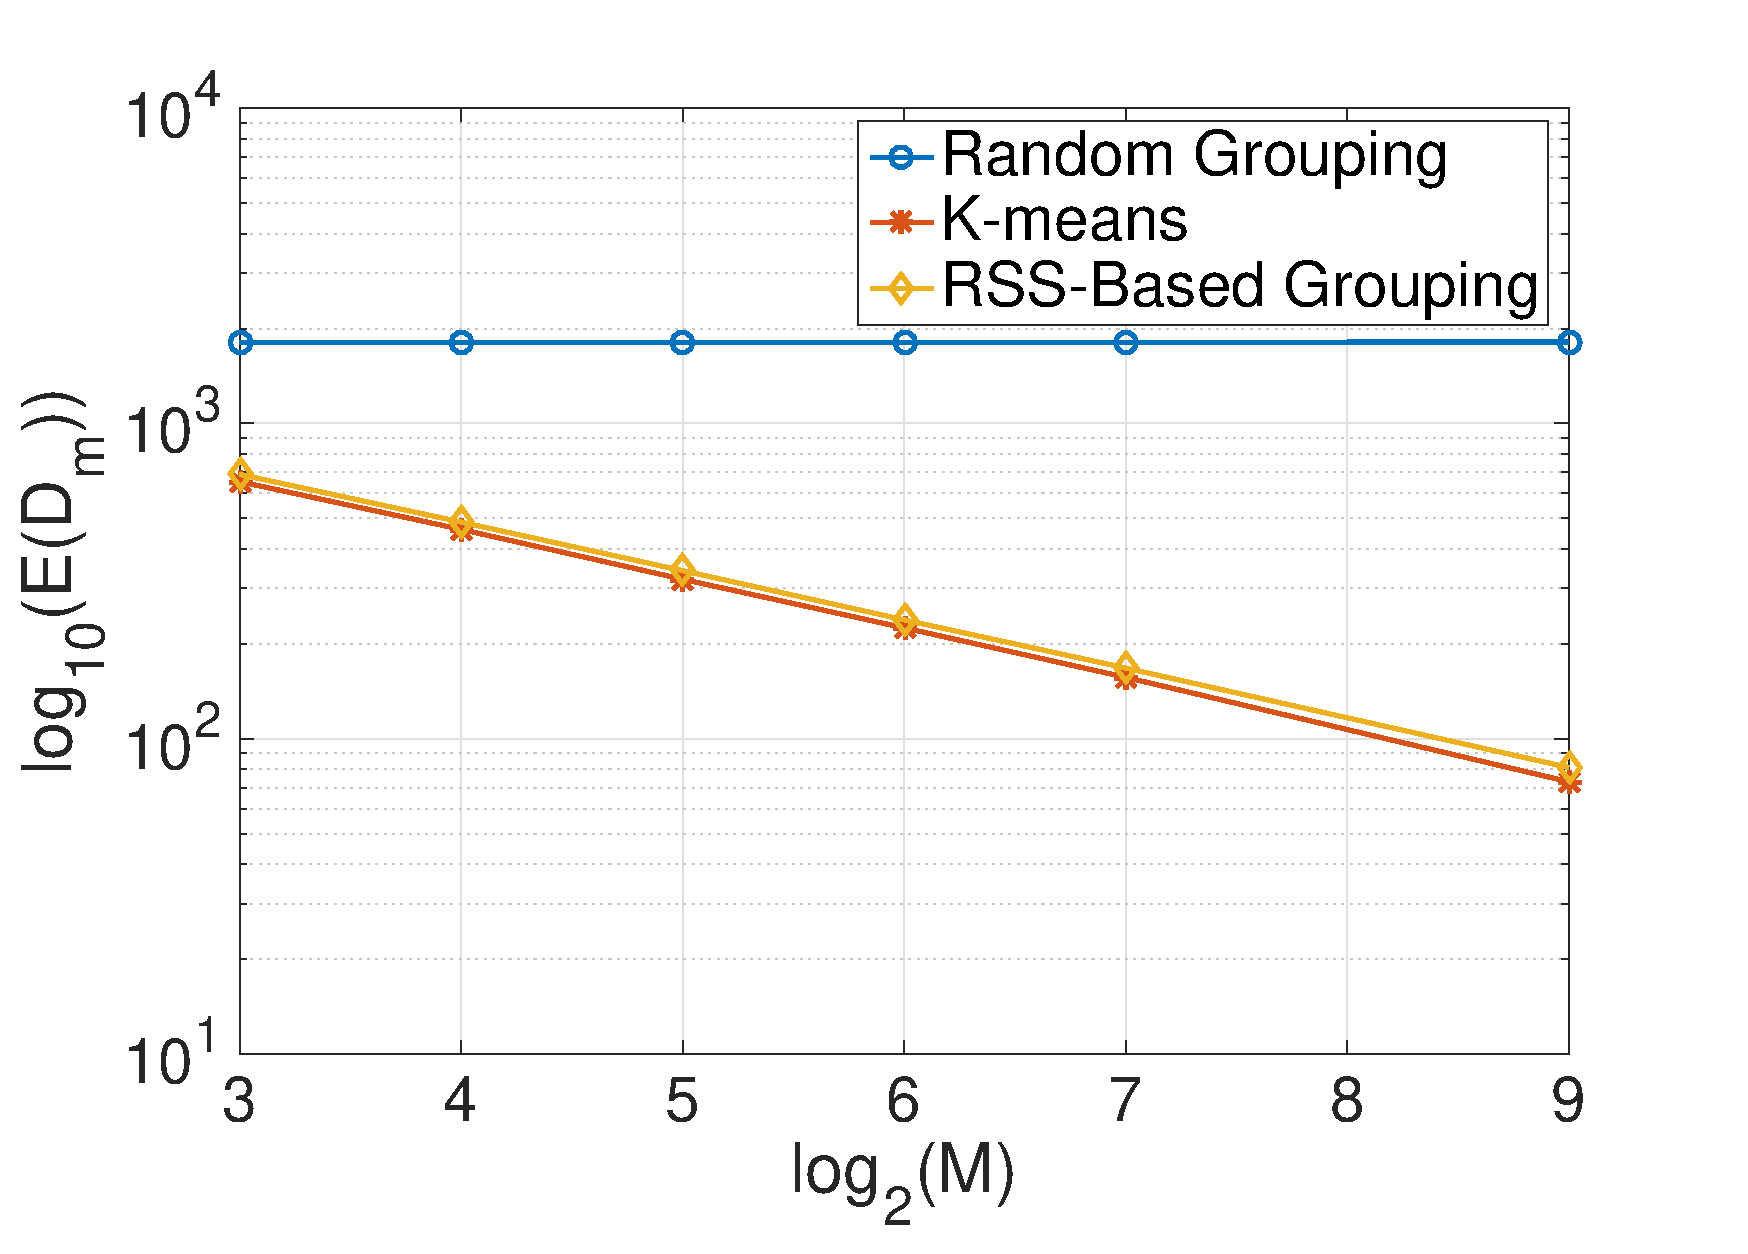
\includegraphics[width=.5\textwidth]{figures/final_metric1}%
  \label{fig:meansum}}
  \subfloat[][Standard deviation of the number of nodes in different groups]{\includegraphics[width=.5\textwidth]{figures/final_metric2}%
  \label{fig:variance}}
  \caption{Grouping performance metrics}
  \label{fig:metricx}
\end{figure}

\iffalse
\begin{figure} 
  \centering
  \includegraphics[width=.95\textwidth]{figures/final_metric2}
  \caption{Simulation result for standard deviation of the number of nodes in different groups}
  \label{fig:didi}
\end{figure}
\fi

%Considering the higher transmission power and the receiving antenna gain at the AP side, we assume that the sensing distance between two user nodes may be equal to or smaller than the maximum transmission distance to the AP.
Assuming that all nodes have the same sensing range, $R_s$, the probability of two random nodes in the same group be in their sensing range versus $R_s$ for a constant number of groups is shown in Fig. \ref{fig:prob}. The figure also shows that the approximation in (\ref{eq:cdf}) not affect the result very much. As we can see in the figure, best performance is for the clustering using the k-means algorithm but the RSS-based grouping scheme also performs very close to the k-means and much better than the random grouping schemes. The same probability assuming Rayleigh fading channel between nodes is also shown in Fig. \ref{fig:prob}. The performance with Rayleigh fading channels is degraded because considering fast fading the areas occupied by groups are no longer Voronoi and the group head with the highest sensed power is not necessarily the closest one. As shown in the figure the algorithm still performs well which indicates that, the RSS estimation accuracy required is low, which results in a small overhead.

With the simulation results following analytical results, our assumption in section \ref{systemdesign} is verified. The simulation and analytical results are closer to each other as M grows. That is because, with a higher value of M, the edge effect becomes more negligible.

%the probability that a node's distance to its group head is larger that R becomes smaller.
%Probability of having hidden terminal versus number of group for a constant range ,for avg-power based and random grouping schemes is shown in figure \ref{fig:prob2}

\begin{figure}
  \centering
  \subfloat[][]{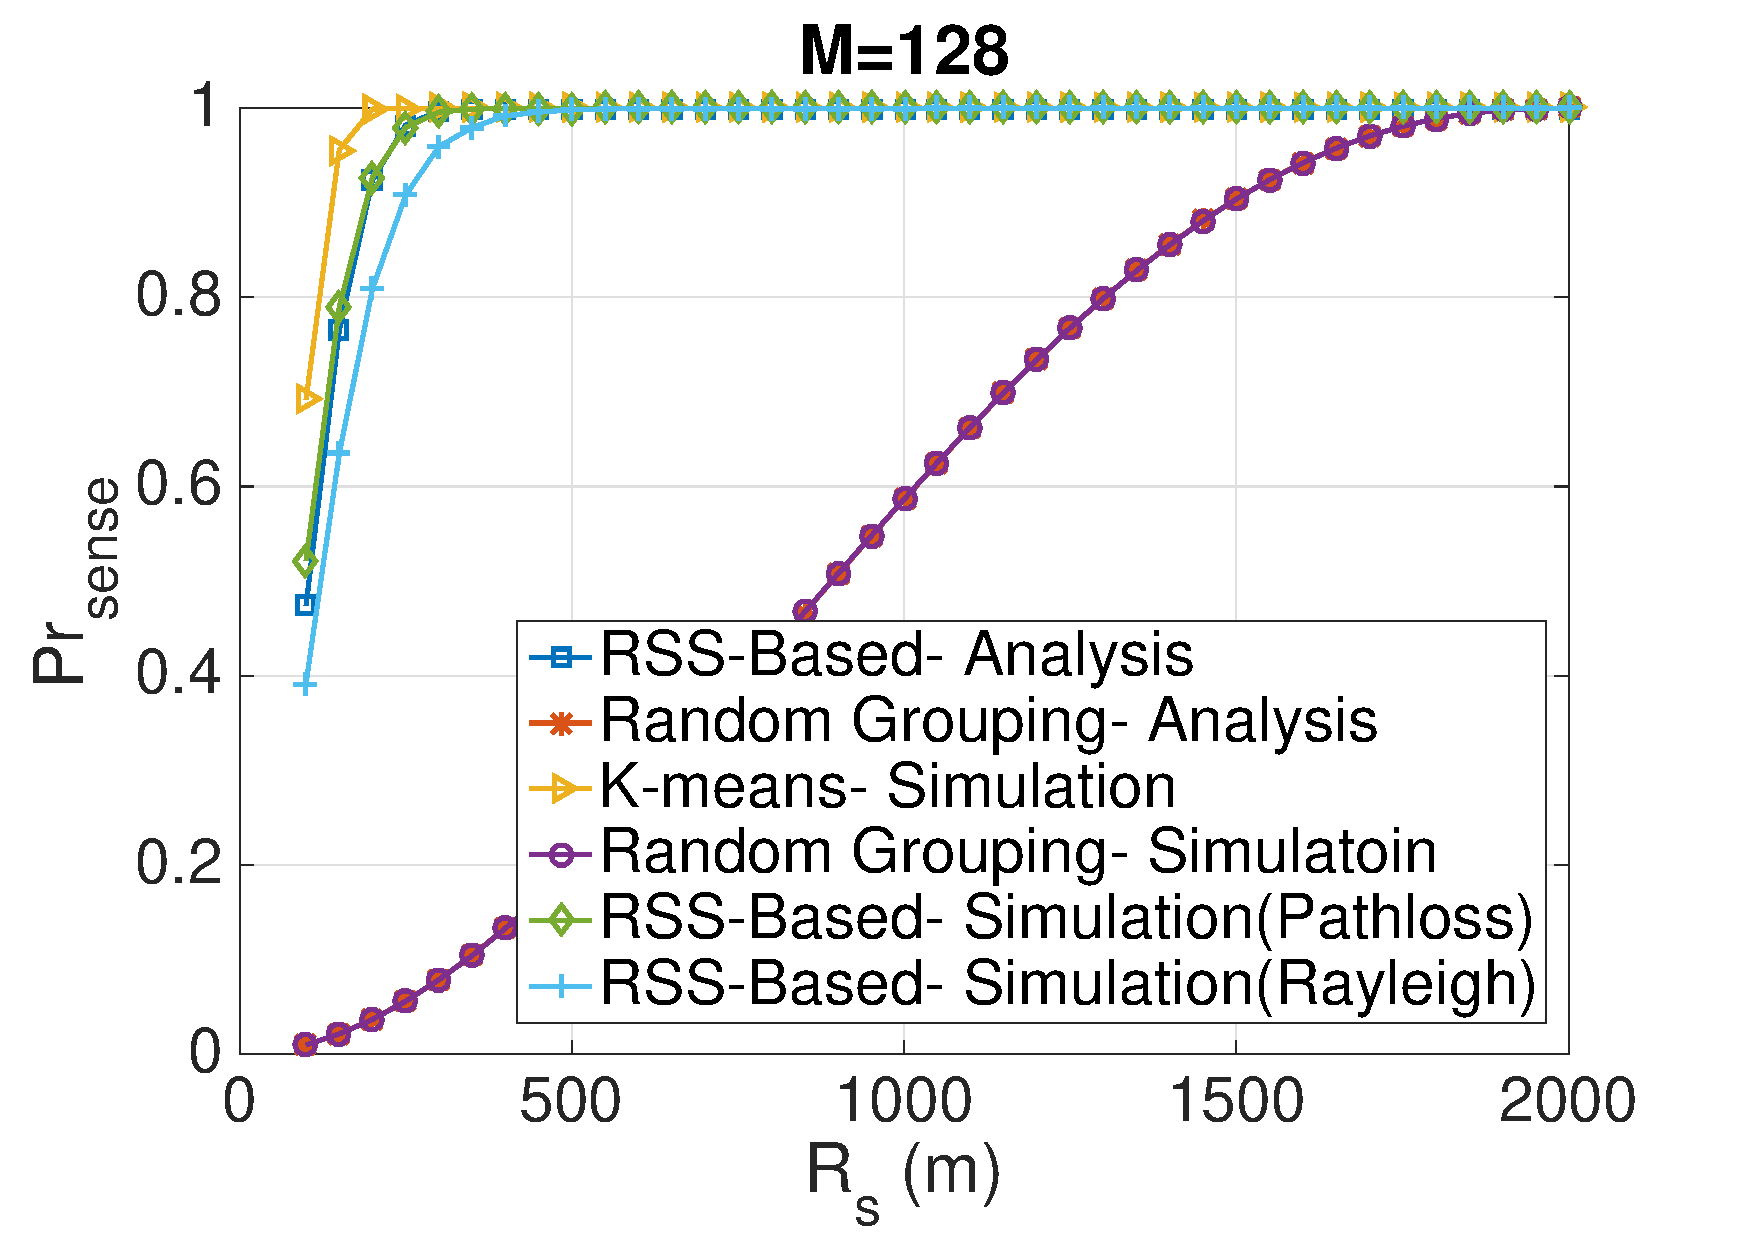
\includegraphics[width=.47\textwidth]{figures/final_probability_fixedM}%
  \label{fig:prob}}
  \subfloat[][]{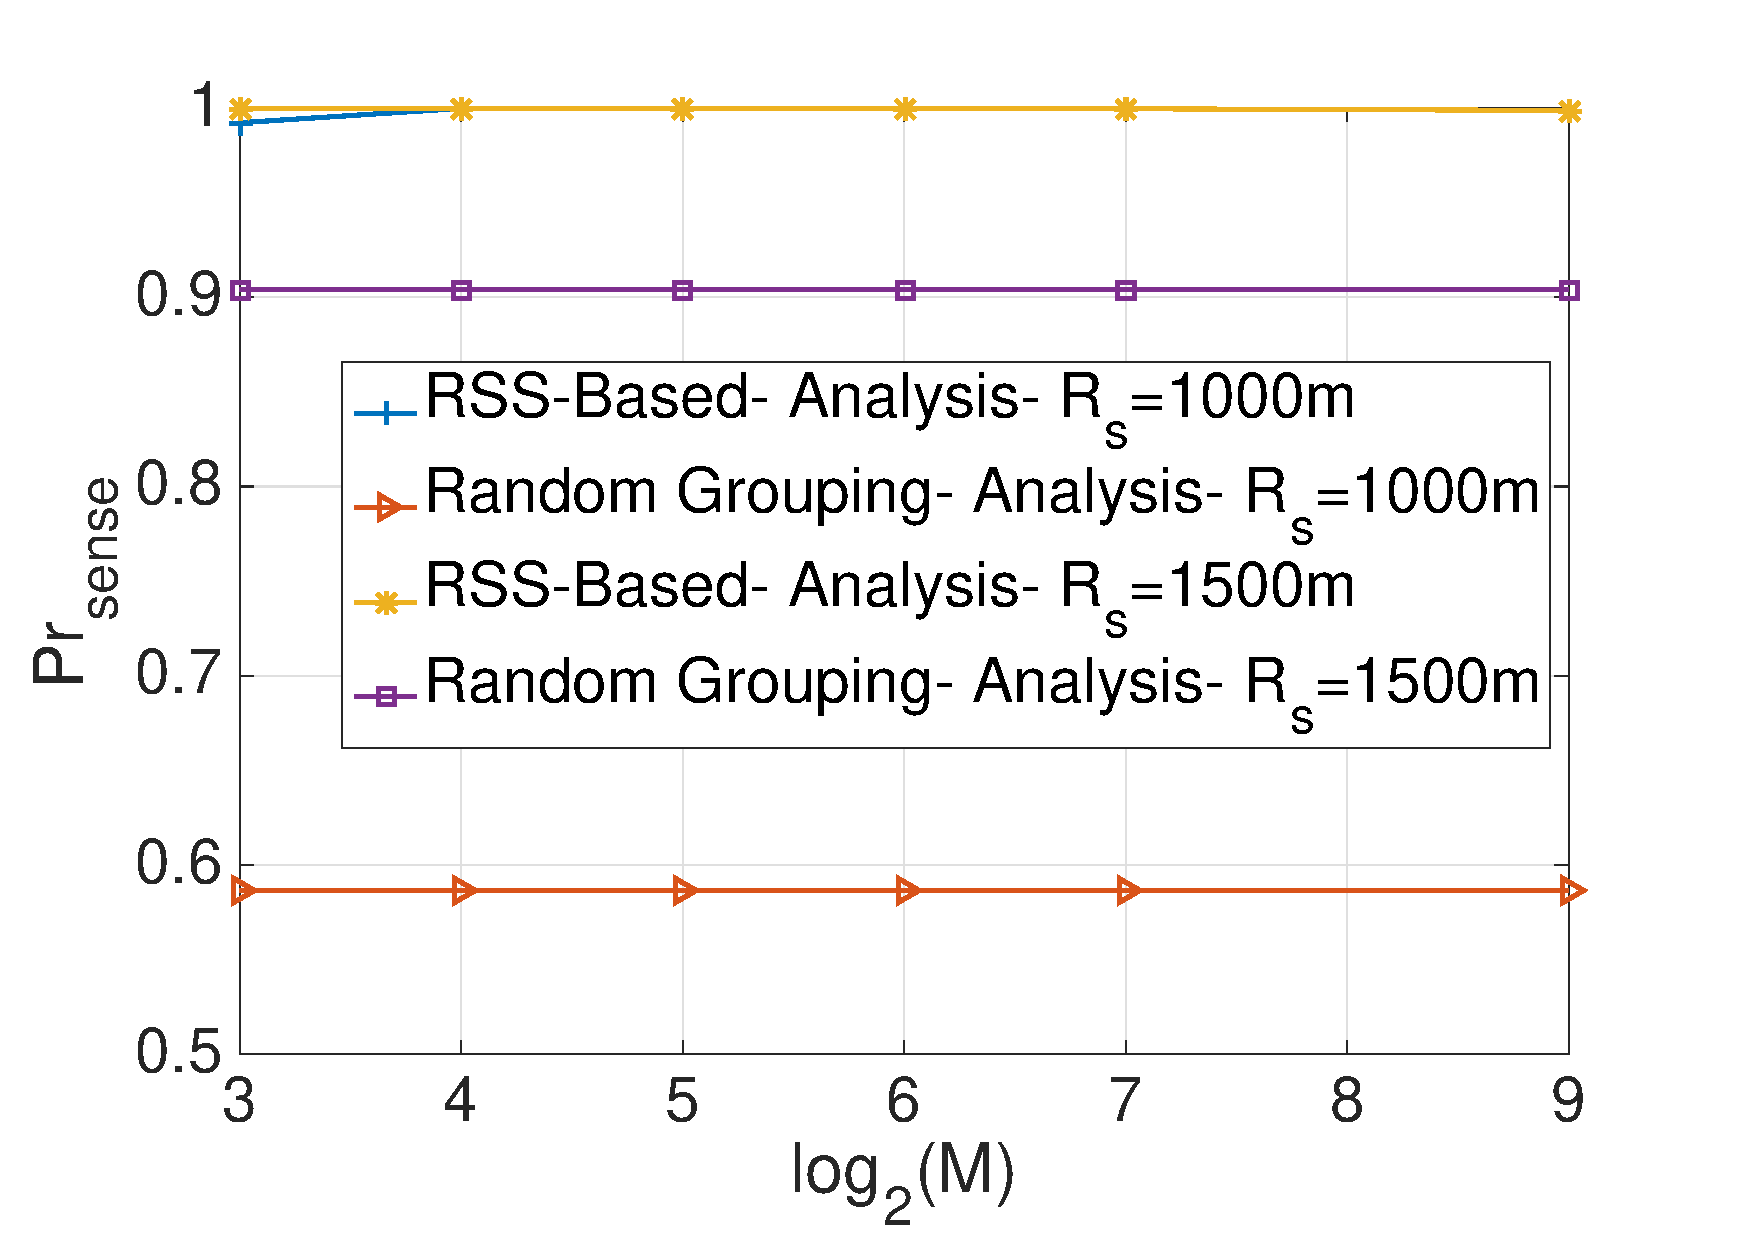
\includegraphics[width=.47\textwidth]{figures/final_probablity_fixedR_analysis}%
  \label{fig:prob2}}
  \caption{Probability of two nodes, within a group, being in the sensing range of each other}
  \label{fig:probabilities}
\end{figure}


\iffalse
\begin{figure}
  \centering
  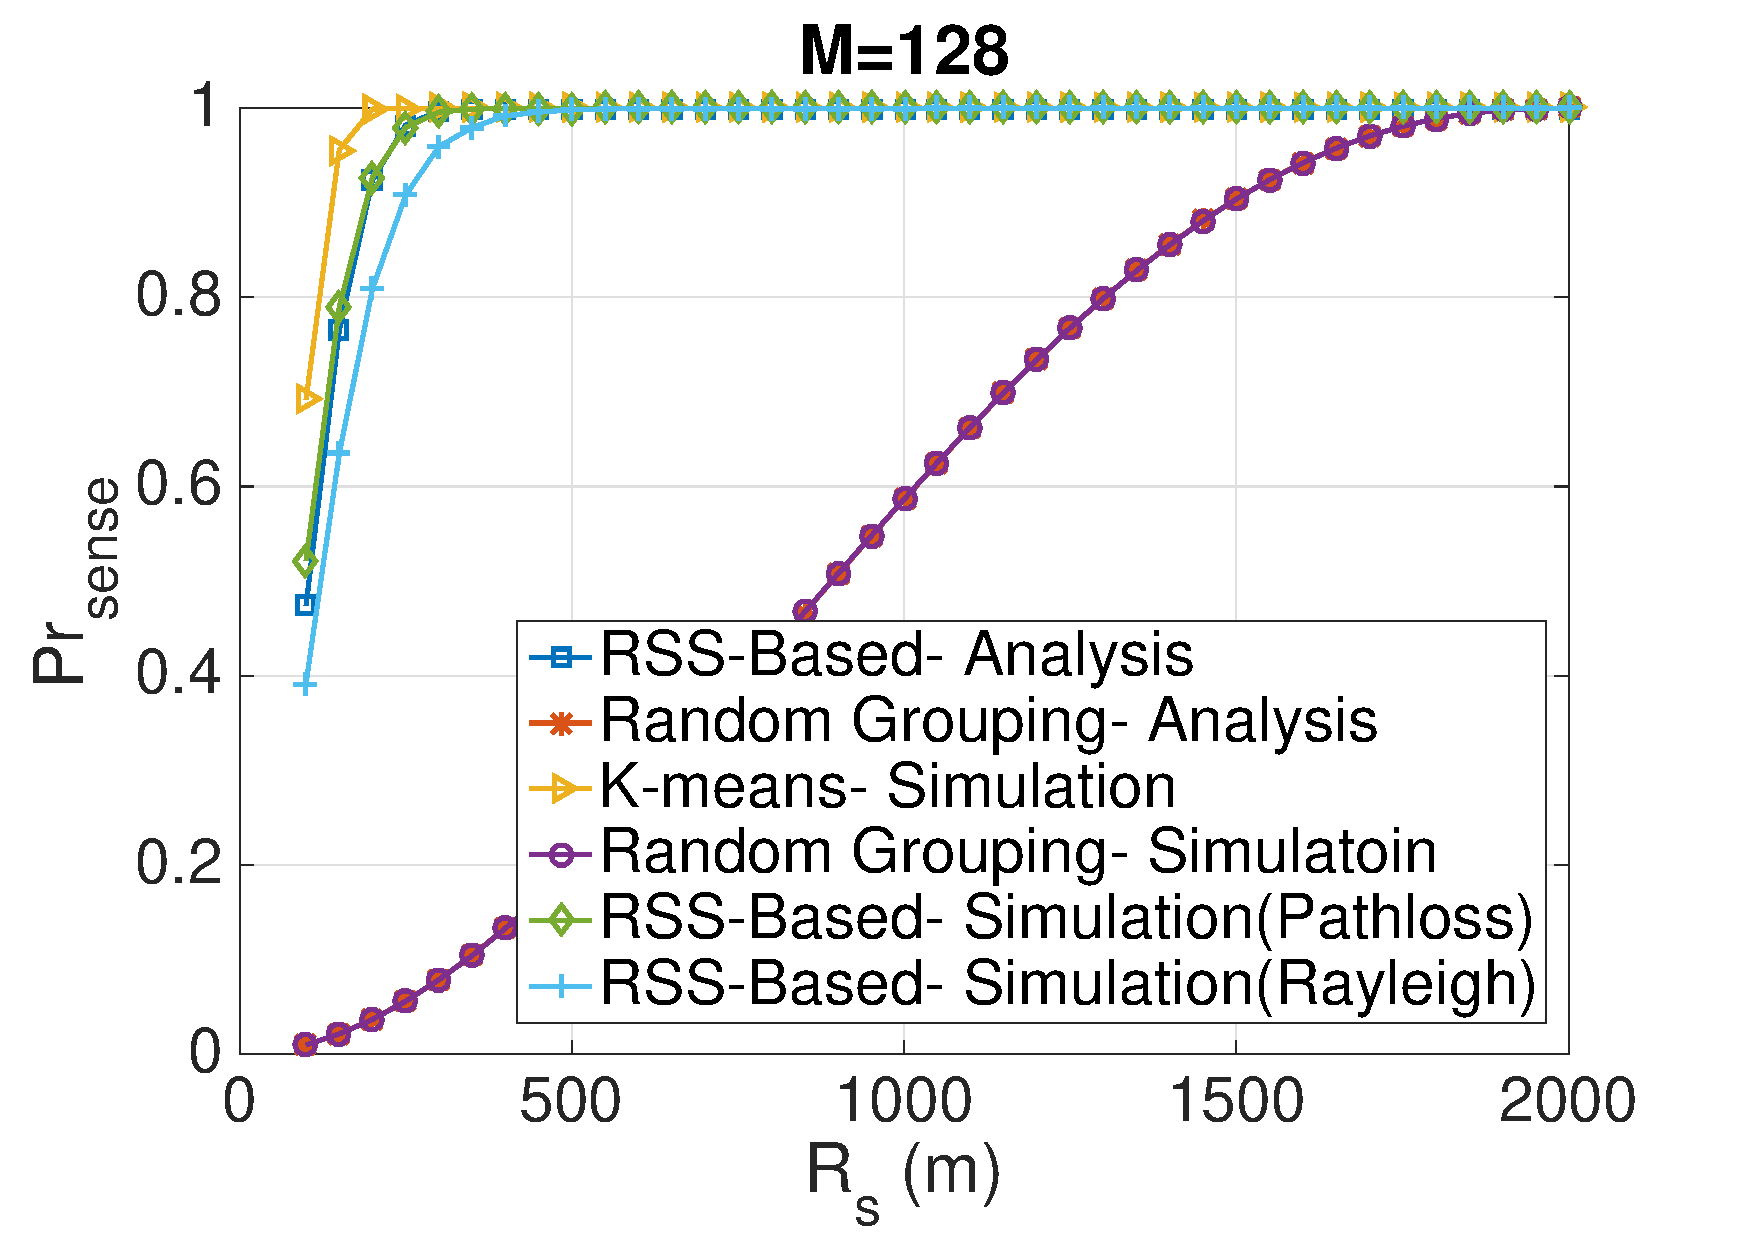
\includegraphics[width=.95\textwidth]{figures/final_probability_fixedM}
  \caption{Probability of two nodes, within a group, in the sensing range of each other}
  \label{fig:prob}
\end{figure}
\fi
Fig. \ref{fig:prob2} shows the probability of two nodes in the same group being in each other's sensing range when all nodes' sensing range is fixed and the number of groups changes. This probability does not change with the number of groups for random grouping because nodes in the same group can still be anywhere in the coverage area and their distance still follows the same PDF. Though in case of the RSS-based grouping algorithm, a larger number of groups results in a higher probability for group members to be in the sensing range of each other because it makes the Voronoi cells smaller.    

\iffalse
\begin{figure}
  \centering
  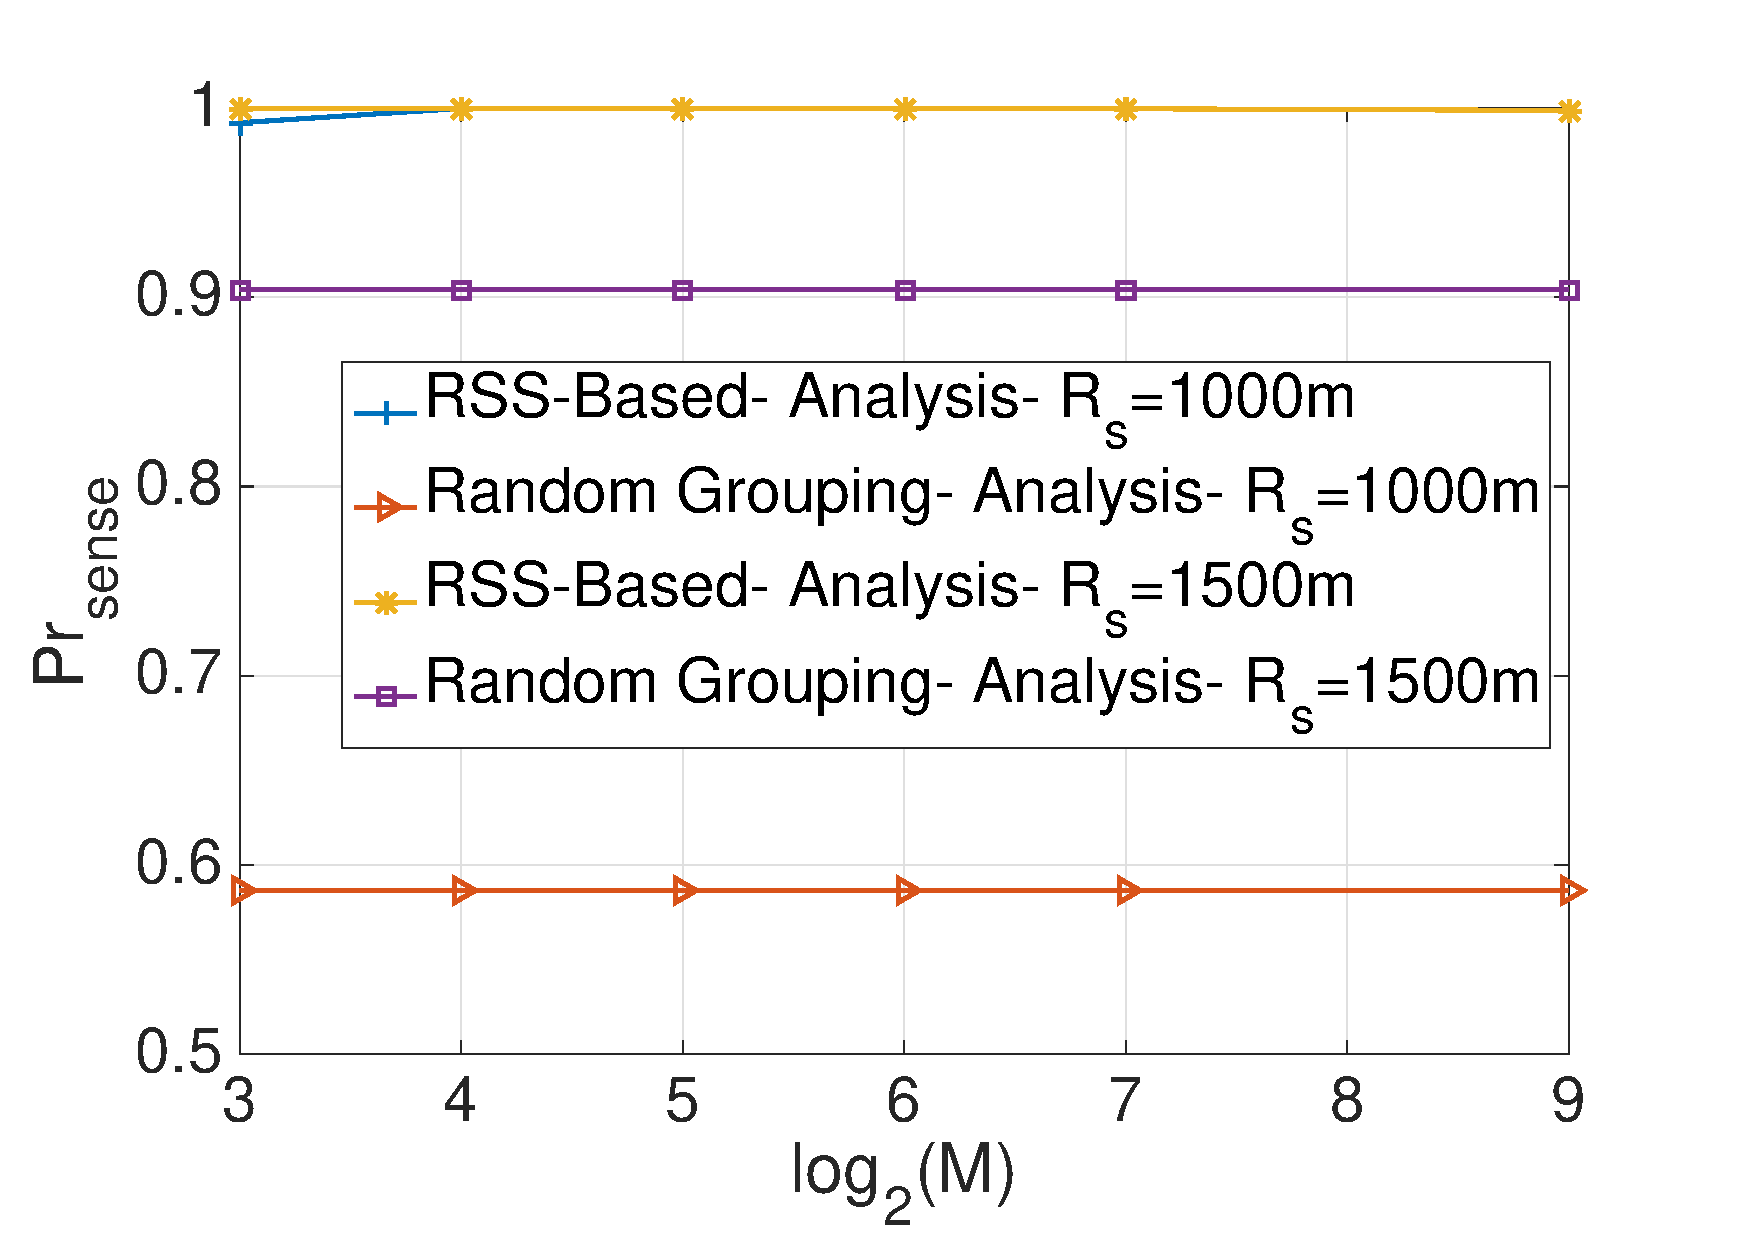
\includegraphics[width=.95\textwidth]{figures/final_probablity_fixedR_analysis}
  \caption{Probability of two nodes, within a group, in the sensing range of each other}
  \label{fig:prob2}
\end{figure}
\fi

Fig. \ref{fig:throughput} shows the throughput simulation result for different grouping schemes along with k-means clustering algorithm using NS-2. Table \ref{table:throughput} shows the parameter setting for simulations used in this section. Other common settings such as PHY and MAC header are set according to the IEEE 802.11 standard \cite{wlan2011}. The payload size is set to be low considering the IoT applications such as smart meter measurement reporting and all nodes are using RTS/CTS mechanism. Only the uplink traffic is considered and a non-collided transmission is assumed to be successful which that means the PHY layer BER is not considered. 

\begin{figure} 
  \centering
  \includegraphics[width=.95\textwidth]{figures/throughput}
  \caption{Throughput of Uplink traffic}
  \label{fig:throughput}
\end{figure}

 In Fig. \ref{fig:throughput}, the throughput for random scheme is very low because the time for a single packet transmission is more than the largest back off window (1024 slots) and almost any transmission would be interrupted when there is a few active nodes who are hidden terminals. In other words, \iffalse in a saturated traffic scenario, \fi a node with a hidden terminal may hardly success in transmitting a packet to the AP without collision.

This figure also shows the limited cost that RSS-based grouping pays due to the higher standard deviation of number of nodes in each group. The throughput using the proposed RSS-based grouping is close to that using the centralized K-mean solution. On the other hand, random grouping has much worse performance due to the hidden terminal problem even when the sensing range is as high as 1500m. Note that the theoretical sensing range without considering the shadowing effect may be much higher than the practical sensing range, so grouping considering the location is important to avoid hidden terminal and improve network performance.


\begin{table}
% increase table row spacing, adjust to taste
%\renewcommand{\arraystretch}{1.3}
%if using array.sty, it might be a good idea to tweak the value of
%\extrarowheight as needed to properly center the text within the cells
\caption{Throughput Simulation Parameter Setting}
\label{table:throughput}
\centering
% Some packages, such as MDW tools, offer better commands for making tables
% than the plain LaTeX2e tabular which is used here.
\begin{tabular}{|c||c|}
\hline
Parameter & Value \\  
\hline
 Slot time & 20 $\mu$S \\ 
 \hline
 SIFS & 10 $\mu$S \\
 \hline
 Payload Size & 64 bytes\\ 
\hline
Data Rate & 1Mbps \\
\hline
$R_s$ & 1500 \\
\hline 
CW min & 31 \\
\hline
CW max & 1023 \\
\hline 
\end{tabular}
\end{table}




\section{SDR Implementation of PNC}
This section, presents the simulation and experimental results for the PNC transmission. Since the real gain of PNC can been seen in multi-hop transmissions, the same implementation is used for measuring performance parameters in a Multi-hop Physical Layer Network Coding (MPNC). The main MPNC network design used for multi-hop experiments is adopted from \cite{zhang2017cross}. Then using asynchronous experiments the same two hop performance parameters are measured for multi-hop PNC too. 

\subsection{Testbed Experiments}

\subsubsection{Experiment setting}
USRP N210 sets with XCVR2450 daughterboards are used to run the PNC experiments. The software used to develop PNC is GNURadio. The transmission gain of transmitting USRPs is set to $18$~dB and the receiver gain of receiving USRPs is set  to $5$~dB. %The distance between devices is 35Cm and 
The carrier frequency is chosen as $2.45$~GHz. The length of the Sync preamble is $64$ symbols and the $SpS$ used in the experiments is four. 
%When the number of hops is larger than two, the experiment is ran in an asynchronous manner in order to have the right SINR.


\subsubsection{BER, two-hop}
To begin with, we first built a two-hop testbed where two sources A and B exchange the information through a relay, as shown in Fig.~\ref{fig:twohoptestbed}. 

Fig.~\ref{fig:e2e_ber} (a) and (b) shows the BER in the MA communications and the end-to-end BER for the two-hop case, respectively. As anticipated, the BER performance deteriorates when the payload length increases, due to the non-stationary wireless channel and the CFOs. Thus, to maintain a low BER,  preambles could be repeated periodically.
%Note that for many machine-type communications with the small-packet feature, packet payload size is quite small, so they fit well with the PNC solutions. 
A somewhat surprising resul in Fig.~\ref{fig:e2e_ber} (a) is that there is a small drop of BER around 150-bit block length. This is because, due to CFO, the phase difference of the two transmissions superimposed at the relay changes periodically. From  Sec.~\ref{sec:e2eberana}, BER with different phase shift is slightly different. After 100-bit was sent, the phase shift returns to the area corresponding to low BER.  %After an entire cycle, it comes close to the signal again.

\begin{figure}
    \centering
    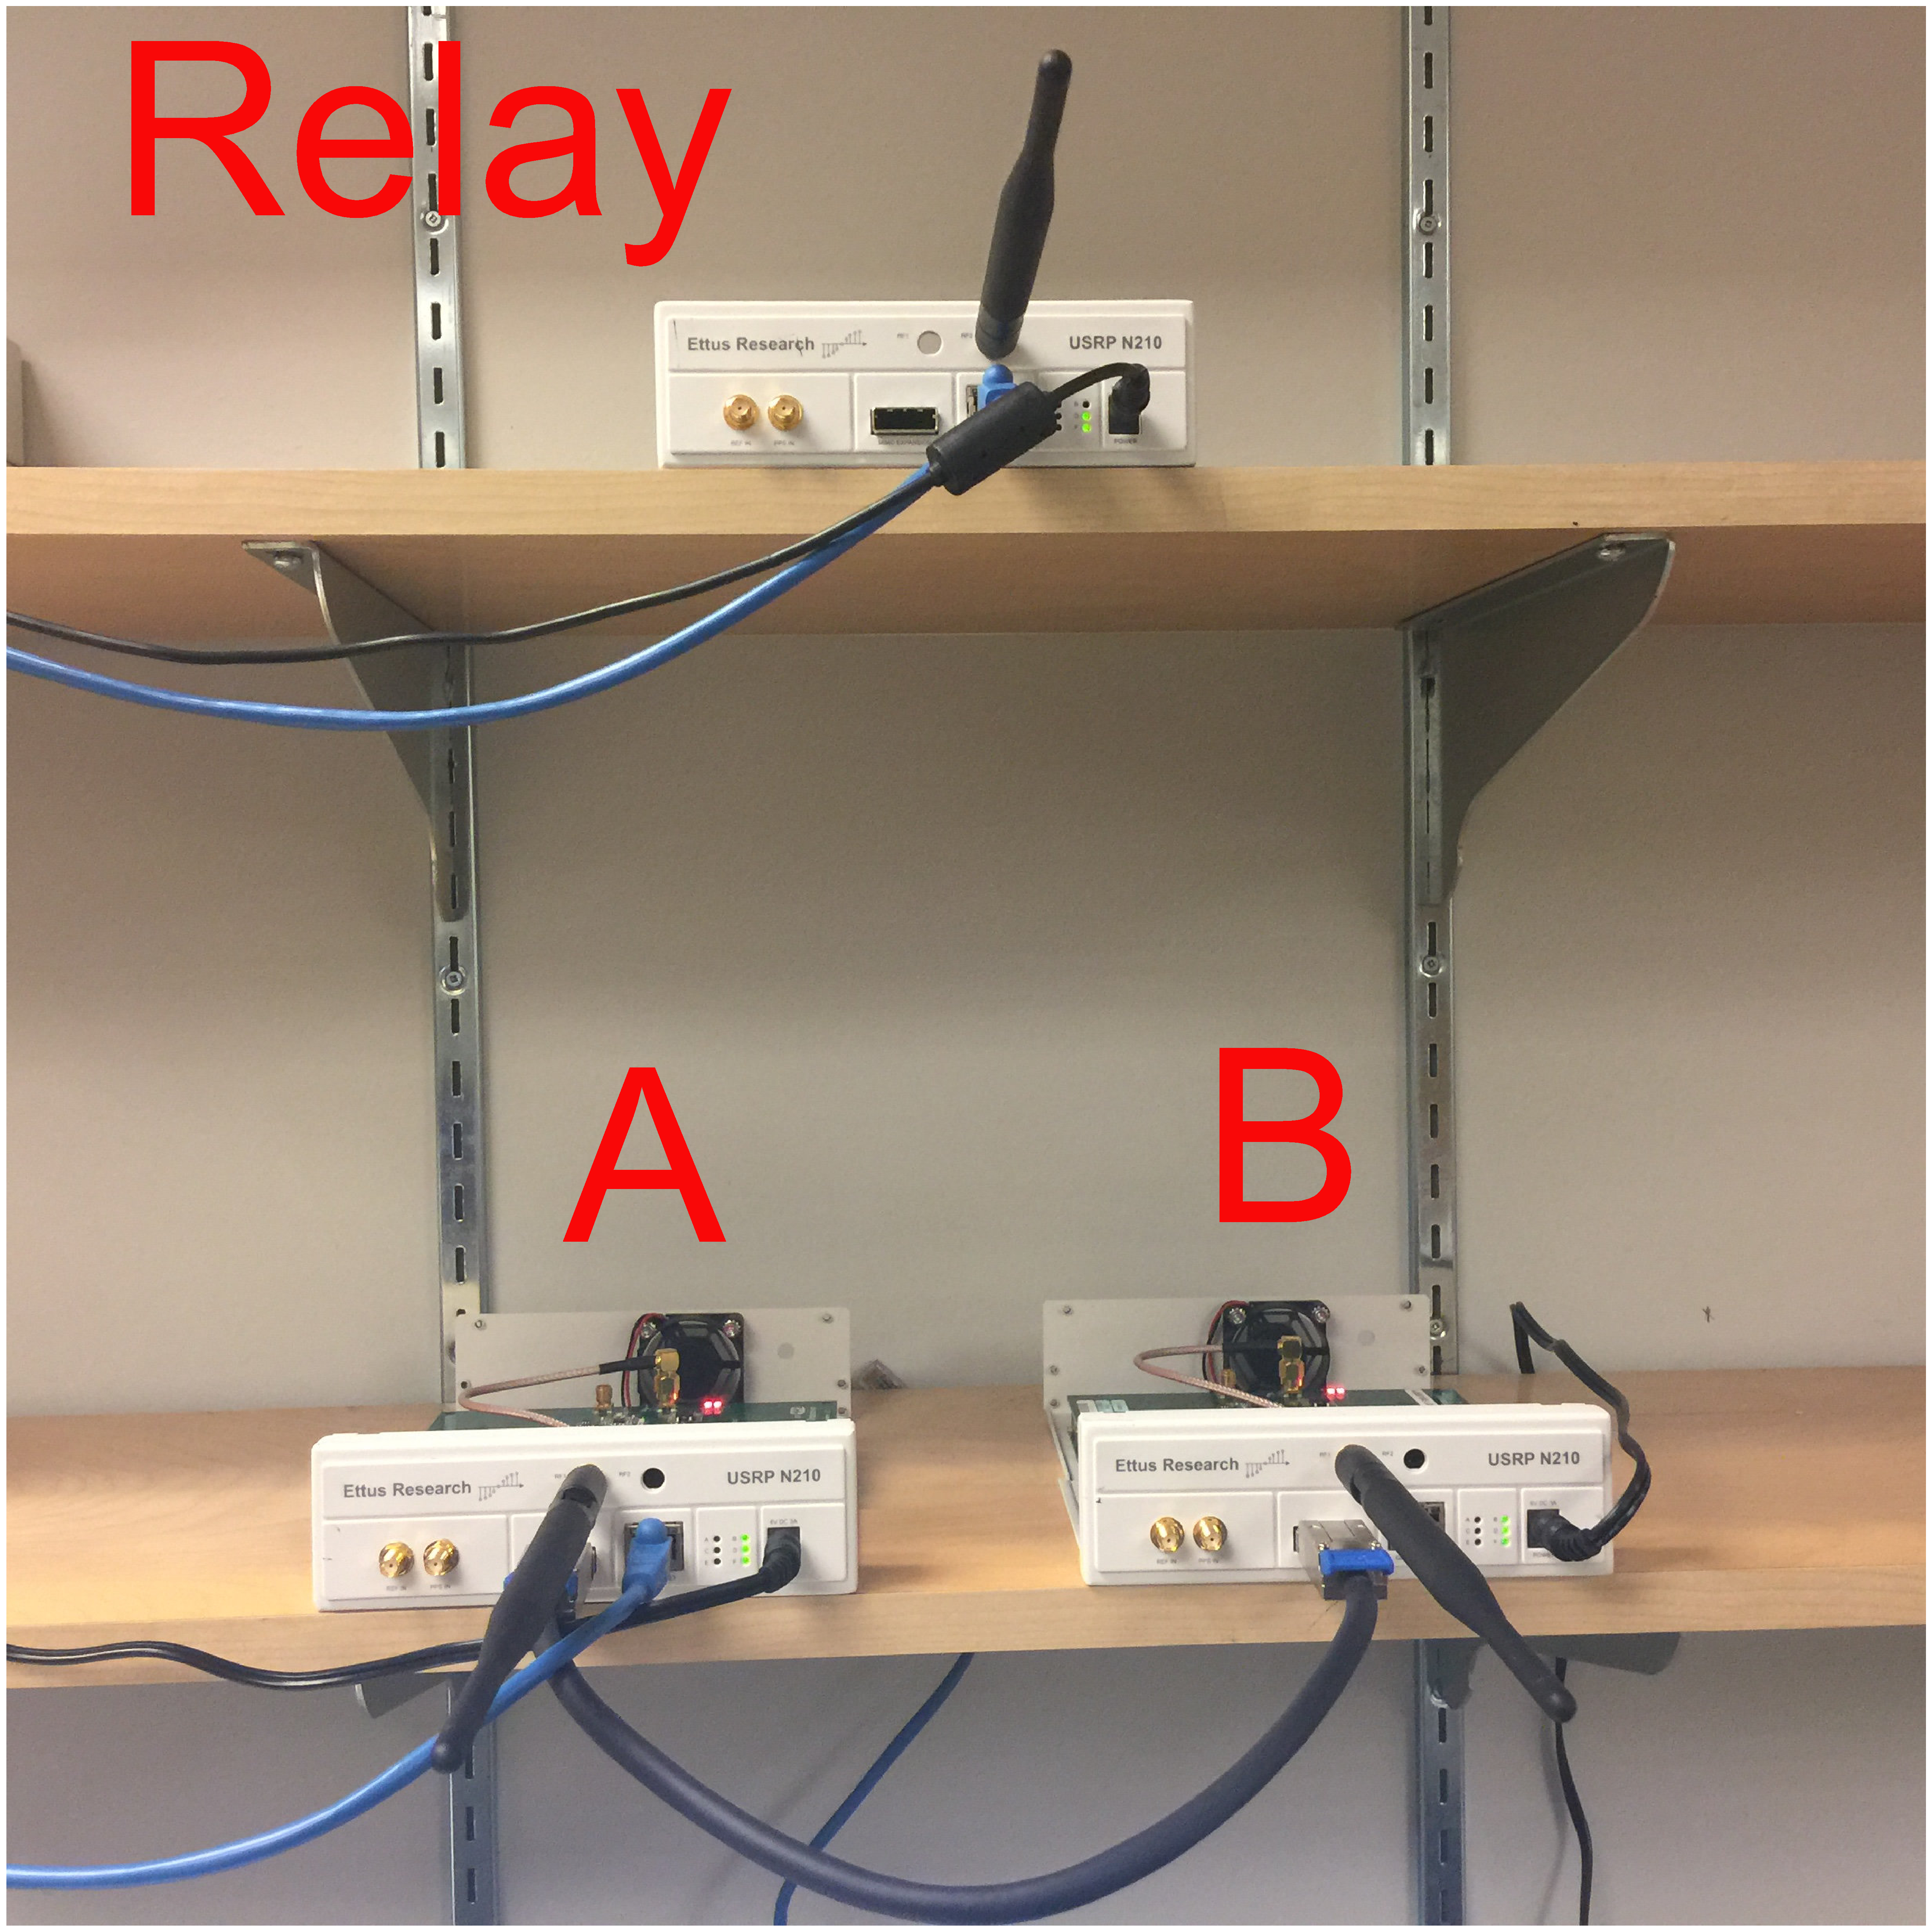
\includegraphics[width=0.95\textwidth]{figures/testbed}
    \caption{Testbed, two-hop scenario.}\label{fig:twohoptestbed}
\end{figure}

%c: mohammad: add the results with 25 bits in. what is the unit of x-axis? bits or bytes? add the unit to the figure.
%                         enlarge the font size 
%                         

%\begin{figure}
%    \centering
%    \includegraphics[width=0.35\textwidth]{figure/cdf}
%    \caption{End-to-end BER, MPNC vs. ANC \cite{katti2007embracing} }
%    \label{fig:cdf}
%\end{figure}

The end-to-end BER results in Fig.~\ref{fig:e2e_ber} (b) include both the MA transmissions and the broadcast transmissions from the relay to the sources. We further compared the end-to-end BER performance of PNC with that of ANC reported in~\cite{katti2007embracing}. The relay in ANC uses an amplify-and-forward approach, instead of the mapping function. From Fig.~\ref{fig:e2e_ber} (c),  MPNC slightly outperforms ANC, from the USRP testbed experiments. In general, the performance of amplify-and-forward degrades in the low SINR region. 

\begin{figure*}
\centering
\begin{tabular}{ccc}
    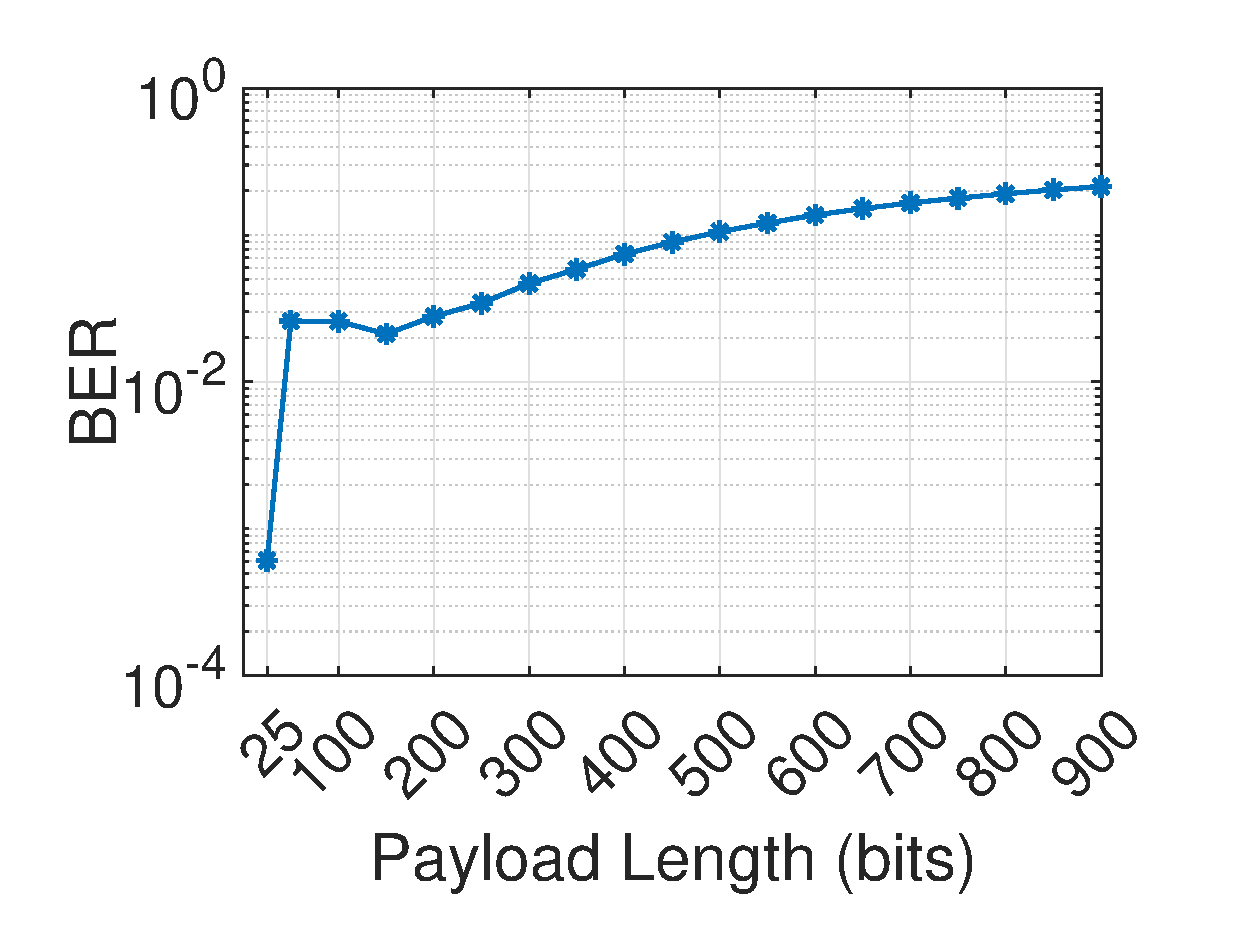
\includegraphics[width=0.33\textwidth]{figures/BER_Payload_MA.eps} &
    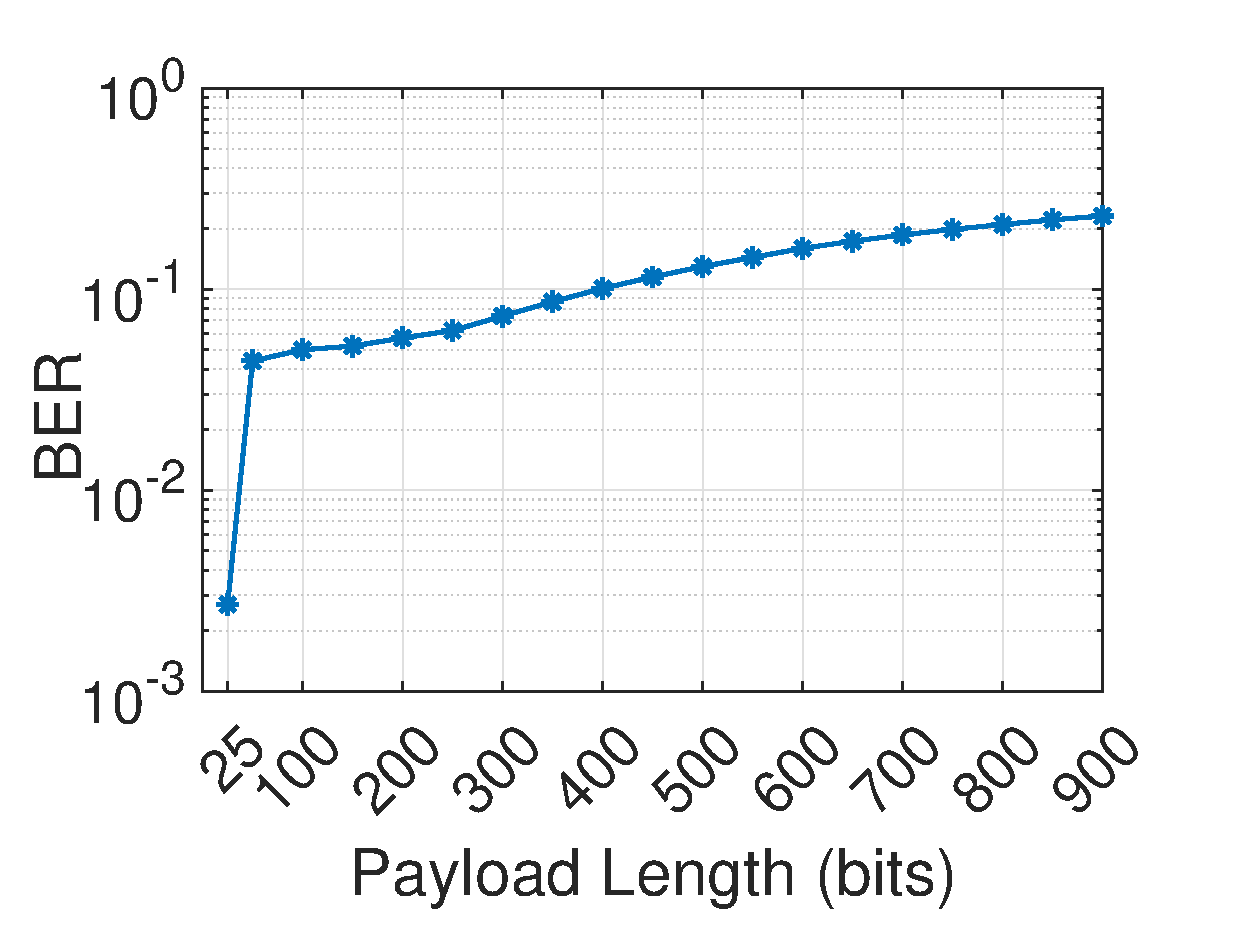
\includegraphics[width=0.33\textwidth]{figures/BER_Payload_e2e.eps}&
     \includegraphics[width=0.33\textwidth]{figures/cdf}\\
      (a) MA  transmission BER &    (b) End-to-end BER & (c) MPNC vs. ANC
      \end{tabular}
       \caption{BER performance, two-hop.}
    \label{fig:e2e_ber}
\end{figure*}

\begin{figure} 
\centering
\begin{tabular}{cc}
   \hspace*{-12pt} 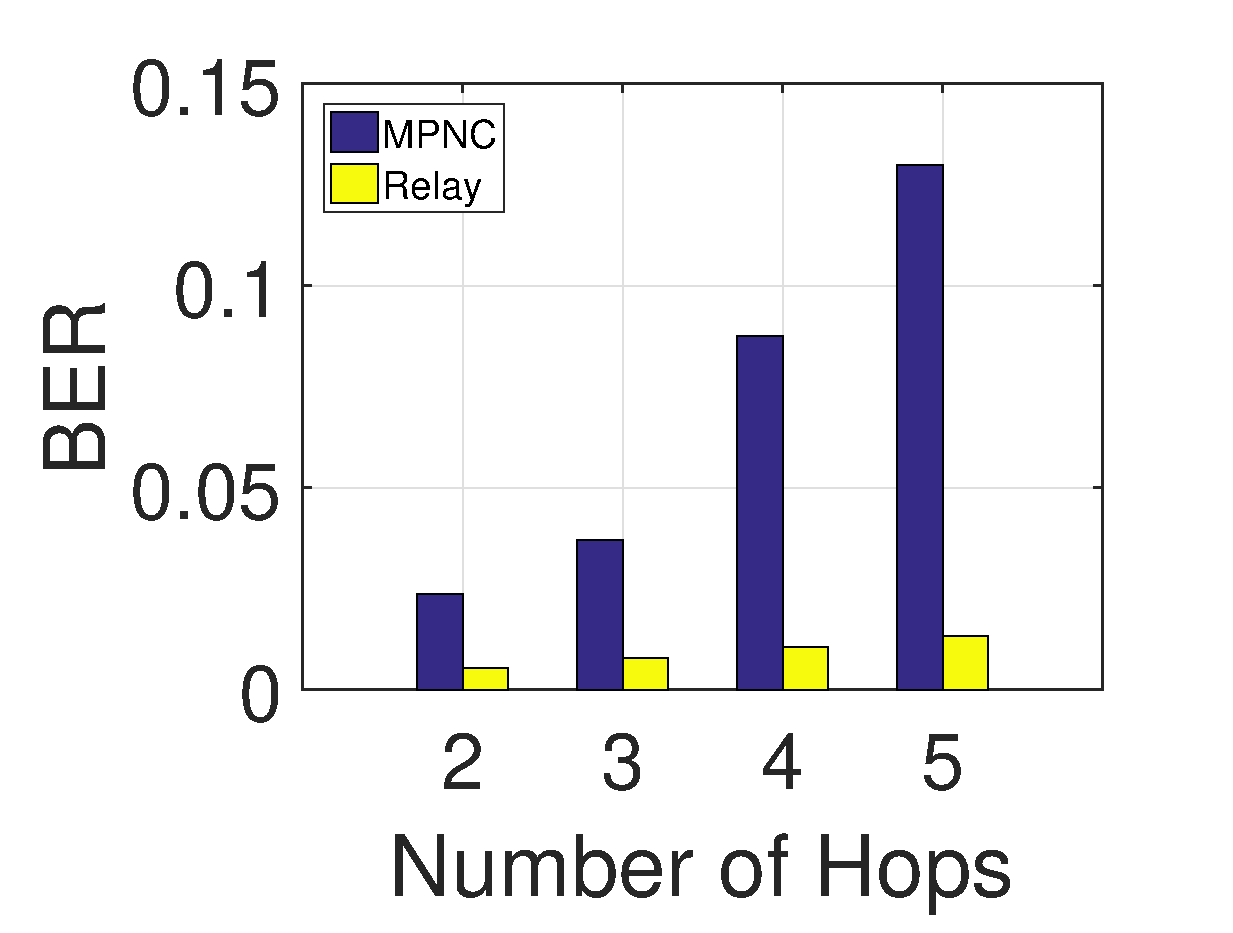
\includegraphics[width=0.47\textwidth]{figures/ber_bar_160}&
   \hspace*{-12pt}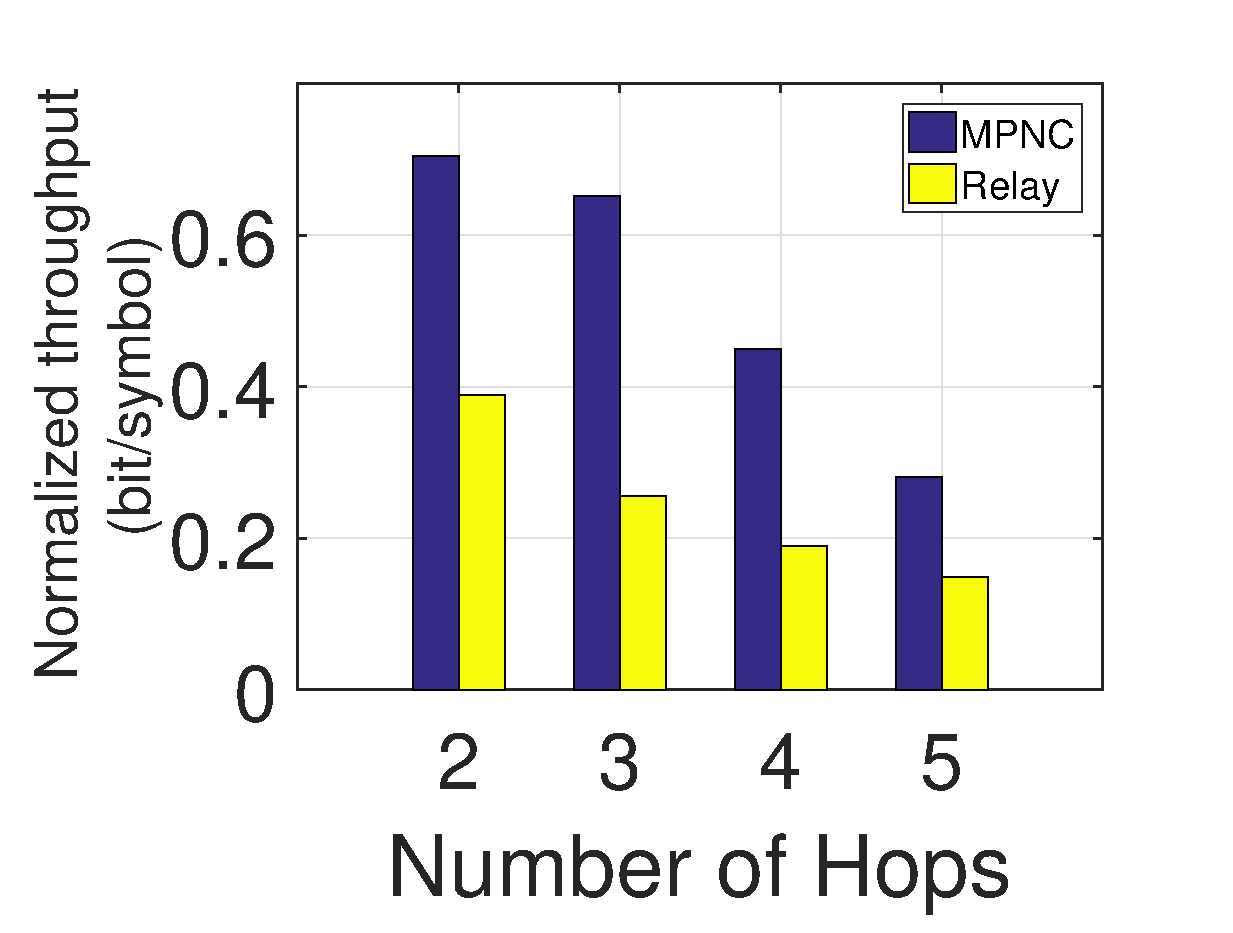
\includegraphics[width=0.47\textwidth]{figures/th_bar_160}\\
      \hspace*{-12pt} (a) End-to-end BER &
 \hspace*{-12pt} (b) Normalized throughput
      \end{tabular}
       \caption{Multi-hop performance. Multi-hop End-to-End BER are calculated using formulations outlined in table 5.1 of \cite{zhang2017cross}.} %(payload = 160 bits)}
    \label{fig:experiment_ber}
\end{figure}

\subsubsection{Multi-hop performance}
Next, we extended the two-hop scenario to multi-hop scenario, where the number of hops varied from two to five. The transmission and reception of the relays for multiple hops behave similarly as that in the two-hop case, except that the mutual interference  and the error propagation problem will lead to a higher BER.

Figs.~\ref{fig:experiment_ber} (a) and (b) compare the end-to-end BER and normalized throughput, respectively of MPNC and that with hop-by-hop relay. 
The normalized throughput is the number of bits successfully received by the destination per symbol duration. 
From the figures, although the end-to-end BER of MPNC is much higher than that of hop-by-hop relaying, due to both the worse BER performance in MA transmissions and the error propagation problem (i.e., a single MA transmission error may affect multiple end-to-end bit errors in a multi-relay path),  the end-to-end throughput of MPNC is much higher
than that of hop-by-hop relay. Using the inexpensive USRP testbed, it is encouraging to notice that the performance gain of MPNC ranges from $75\%$ to $80\%$ for the two- and five-hop cases, and around $150\%$ for the three- and four-hop cases. 


%comparing the two graphs reveals that although end to end BER of MPNC can go much higher than hop by hop relaying, due to its nature of exchanging two packets in two slots with any number of hops, it can always maintain a throughput higher than hop by hop relaying. The throughput of MPNC is also compared to other mechanisms of multi-hop relaying in \ref{sub:throughput} using simulation results.

  



%%%%%%%%%%%%%%%%%%%%%%%%%%%%%%%%%%%%%%%%%%%%%%%%%%%%%%%%%%%%%%%%%%


\subsection{Simulation Results}

To evaluate and compare the performance of the proposed MPNC in controllable and repeatable environment with a wide range of settings, we used Matlab and GNURadio to conduct extensive simulations and the results are presented in this section. 

%In this section, the performance of the proposed multi-hop PNC scheme is evaluated using excessive simulations. Also the effect of multiple parameters that are not controllable in practice is studied. Matlab and GNURadio are softwares used to run simulations. 

\iffalse

\subsubsection{Different number of hops} % (fold)
\label{sub:awgn}
In this subsection, we study the end-to-end performance considering different number of hops, aiming to identify the optimal number of hops. 
For fair comparison, here, we let the total transmission power in any two continuous slots be $2E_b$, and all the nodes equally share the total transmission power. In other words, if the number of hops increases, the transmission power per node decreases accordingly. The nodes are located in a linear topology with equal distance for each hop.  The average received SNR of all links are proportional to $d^{-\alpha}$, where $d$ is the hop distance. %We studied the performance of MPNC under AWGN channel with different path-loss parameters.

\begin{figure*}
    \centering
    \subfloat[][$\alpha = 4$.]{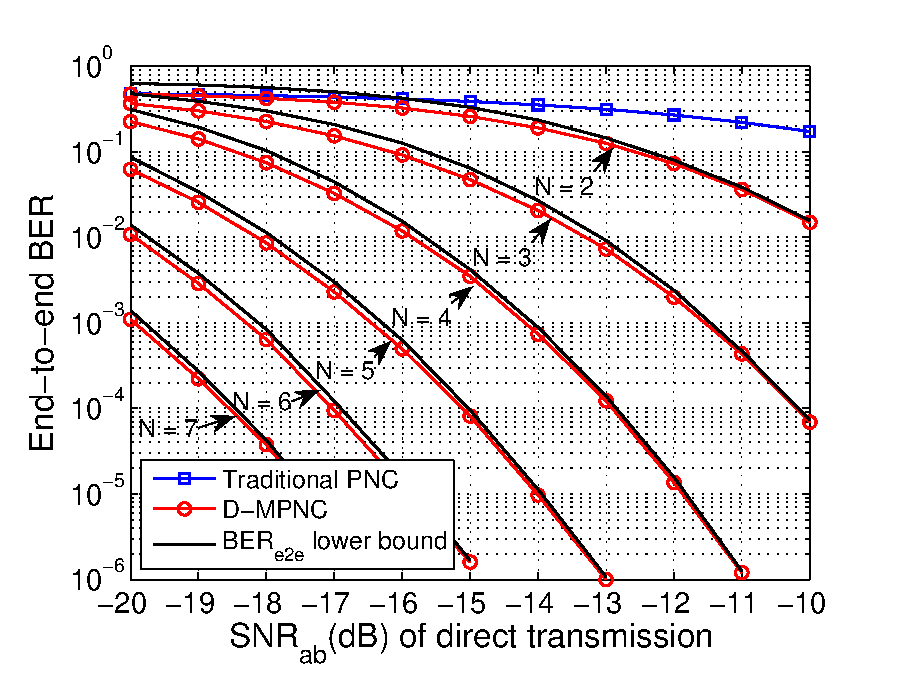
\includegraphics[width=.34\textwidth]{figures/dmpnc_alpha_4_awgn.eps}}
    \subfloat[][$\alpha = 3$.]      {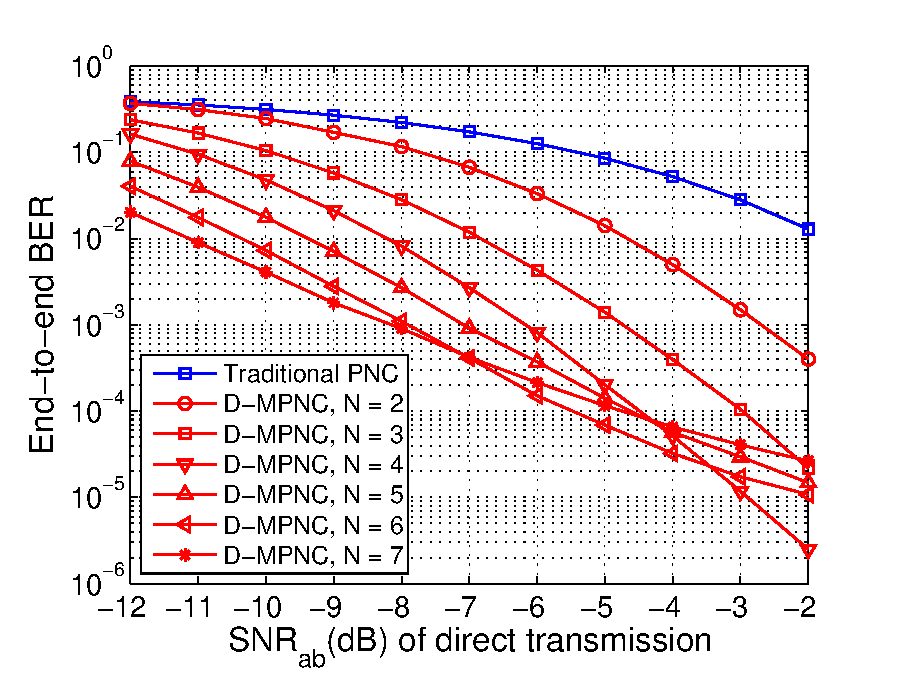
\includegraphics[width=.34\textwidth]{figures/dmpnc_alpha_3_awgn.eps}}
    \subfloat[][$\alpha = 2$.]      {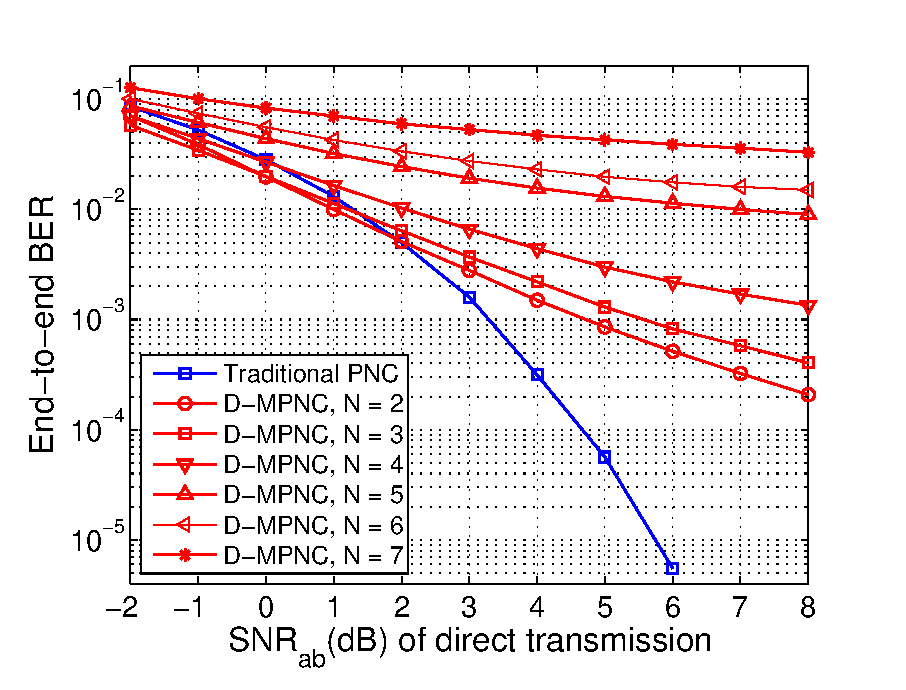
\includegraphics[width=.34\textwidth]{figures/dmpnc_alpha_2_awgn.eps}}
    \caption{End-to-end BER performance of MPNC under AWGN channel.}\label{ber-D-MPNC}
\end{figure*}
%c: haoyuan: change D-MPNC to MPNC in the figures, and change "lower bound" to "bound". 

Since the end-to-end data exchange rate of PNC and MPNC remains the same no matter how many relays are used, we only need to compare the end-to-end BER performance. 
The end-to-end BER results considering different number of relays and different path loss exponents are shown in Fig. \ref{ber-D-MPNC}. The X axis is the end-to-end $\text{SNR}_{ab}$(dB) by direct transmission (without any relay). The "Traditional PNC" curves are for the case with one relay only so the traditional PNC solution can be directly applied. 
With $N$ relay(s), the transmission power per node is  less while the path loss also reduces. The mutual interference also increases when the number of relays increase. Therefore, there is a tradeoff, and the optimal number of hops largely depends on $\alpha$, typically  ranging  from $2$ to $6$~\cite{goldsmith2005wireless}. 
%Given the end-to-end $\text{SNR}_{ab}$(dB) in (\ref{end-to-end-snr}) and the distance $d$(m) between the sources, the larger $\alpha$ is, the SINR(dB) of each hop in (\ref{sinr}) is larger by shortening the transmission path. Another impact is that a larger $\alpha$ reduces the impacts of the inference from other transmitting nodes to the receiver due to a larger path loss. The impacts of the path-loss parameter $\alpha$ is also studied in this section.

In Fig. \ref{ber-D-MPNC}(a), the black curves are the  end-to-end BER bound of MPNC obtained in Table~\ref{L_D_MPNC} and the red circled curves are the simulation results. When the BER is low, the bound and the simulation results converge. This is because,  when the BER is low, the probability that  more than one multi-access and single-hop errors occur in a slot becomes negligible. Comparing Figs. \ref{ber-D-MPNC}(a), (b) and (c),  $\alpha$ has a great impact on the end-to-end BER performance. In Fig. \ref{ber-D-MPNC}(a), when $\alpha=4$, MPNC outperforms the traditional PNC with single relay significantly due to the a relatively larger SINR between the neighbor nodes as the interference and signal strength both decay fast with distance. The tendency also shows that with the lower end-to-end SNR (or larger distance between the sources), we can add more relays to ensure that the BER is below a threshold.
In Fig. \ref{ber-D-MPNC}(c), when $\alpha=2$, the two-hop PNC achieves the best performance when the end-to-end SNR is above $2$~dB; and below that, all solutions perform poorly.  
In Fig. \ref{ber-D-MPNC}(b), when $\alpha=3$, the optimal number of relays depends on the end-to-end SNR (or distance). 
%In Figs. \ref{ber-D-MPNC}(b) and (c), with the increase of end-to-end $\text{SNR}_{ab}$(dB), the end-to-end BER performance converges with a larger relay number $N$. Because the interference from other transmitting nodes in multi-hop PNC also increase with the increase of $\text{SNR}_{ab}$(dB), and the SINR of two neighbor node approach to the upper bound. Further increase $\text{SNR}_{ab}$(dB) will not help to improve the end-to-end BER, as the SNR of each hop is upper bounded by $10\alpha\log_{10}{3}$(dB) as explained in Sec. \ref{sec-inter}.
The results suggest that when $\alpha$ is large (e.g., $\ge3$), we can apply MPNC to solve long-distance wireless transmissions using a large number of relay. 

\fi




\subsubsection{Goodput performance comparison} % (fold)
\label{sub:throughput}


In this section, the goodput of MPNC is studied and also compared with the other state-of-the-art solutions. As we compare the performance of different solutions with the same number of hops, different from the last subsection, here, the transmission power of each node and the hop distance remains constant. %For MPNC, Hop by hop, and Full Duplex solutions, we
The goodput measures the number of error-free packets received per slot.
% is defined as 
%\begin{equation}
%   Th=1-(1-BER)^{Payload Length}\frac{2}{S_k},
%\end{equation}
% where $S_k$ is the number of slots required to exchange $k$ packets. 
For the full-duplex relay solution, in the simulation, we made a strong assumption that the self-interference can be fully cancelled. Thus, the performance shown in our simulation can be viewed as the upper bound of it. 
As the existing PNC method for multi-relay path suffers from the infinite error propagation problem, to make it usable, after detecting each error, the destination must  notify all other nodes and the pipeline should be   flushed and restarted. The goodput for the PNC method is thus affected by the restarts.
Note that with the infinite error propagation problem, an error detection coding have to be used for PNC, but the error correction coding cannot be applied, which is a severe disadvantage for it. 
 
% calculated by
% \begin{equation}
%   Th_{PNC}\sum_{k=1}^{\infty} \frac{2k}{S_k} P_{s,k}^{PNC} P_{e}^{PNC},
% \end{equation}
% where $P_{s,k}^{PNC}$ the probability of successfully exchanging $k$ packets using PNC method and $P_{e}^{PNC}$ is the probability of an error happening while exchanging two packets.


The goodputs  are shown in Fig.~\ref{fig:throughputPNC}. Comparing with the other state-of-the-art algorithms, MPNC has always a higher goodput and can maintain its performance as the number of hops increases. The goodput gains of MPNC over hop-by-hop relay, full-duplex, and PNC is about 3x times, $33\%$, and $68\%$ when the number of hops is as high as eight. Also, from the figure, the goodput of MPNC remains close to 0.9 packet/slot when the number of hops varied from two to eight, showing that it is quite scalable to long paths. 

% subsection throughput (end)


\subsubsection{Effect of CFO on BER} % (fold)
\label{sub:effect_cfo_on_ber}
Fig.~\ref{fig:cfo} (a) shows the impacts of CFOs on the BER performance.
 High CFO is set according to the practical number measured from the USRP devices in our testbed, and the low CFO is 0.1 of that. As it can be seen in the figure, CFO compensation is crucial to the performance of MPNC. The figure shows that when CFO is not compensated, the performance is poor (larger than $10\%$ bits in error) no matter whether the CFO is high or low. On the other hand, using the proposed CFO compensation algorithm can improve the BER performance significantly.

 %Average CFO compensation is when the average value of CFO is used for both $f_1$ and $f_2$.
 % The key result is that although estimating CFO of both nodes with their average and attempting to remove its effect by a multiplication can have a good performance with low CFO values, the algorithm proposed in this paper can maintain a better and lower BER as payload %length increases. The reason for that is because the average CFO method does not remove the effect of CFO completely and a small rotating phase remains in both signals which causes a higher number of errors for large payload lengths.

\begin{figure}
    \centering
    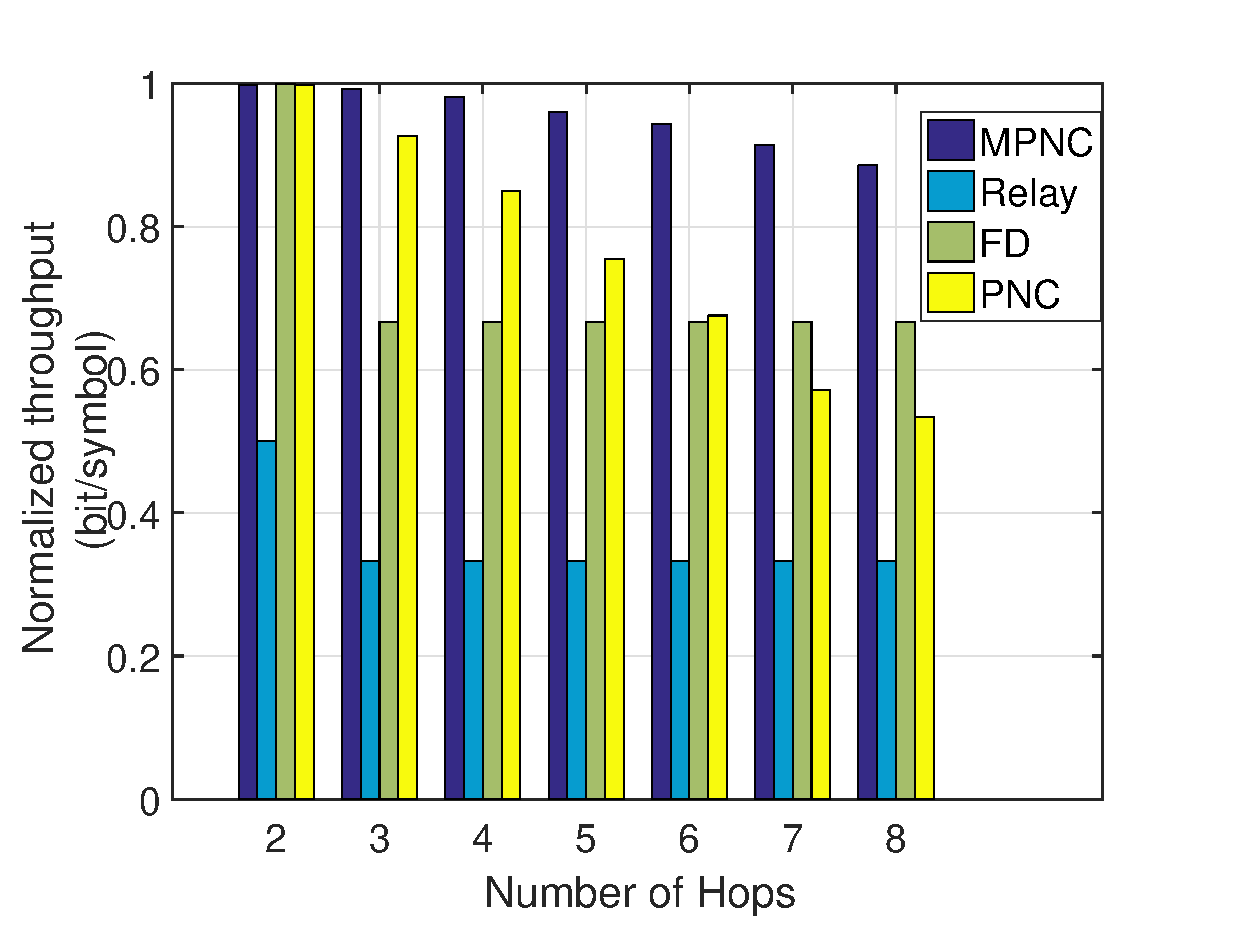
\includegraphics[width=0.95\textwidth]{figures/sim_th_alpha4_snrh2h9BL256}
    \caption{Goodput, per-hop SNR $=9$, $\alpha=4$, Payload=$256$ bits.}
    \label{fig:throughputPNC}
\end{figure}

% subsection effect_cfo_on_ber (end)


\subsubsection{Effect of Channel Estimation Error on BER} % (fold)
\label{sub:effect_of_channel_estimation}
We studied the effect of channel estimation error %which can also be interpreted as having relays on not perfect location, 
on end-to-end BER performance. In Fig.~\ref{fig:cfo} (b), $\delta$ represents the ratio of estimated channel gain and the real channel gain. From the figure, 
overall, the BER increases when the channel estimation error increases,  while  the algorithm can maintain a reasonable BER even with $10\%$ to $20\%$
estimation errors. 
%\begin{figure}
%    \centering
%    \includegraphics[width=0.25\textwidth]{figure/locations2_new}
%    \caption{Effect of Channel Estimation Error on BER}
%    \label{fig:channel_estimation}
%\end{figure}
%c: instead of using alpha, which has been used as path loss exponent, use $\delta$ here. 
% why the 0.8 curve and 0.9 curve cross at 100 bit? 

% subsection effect_of_channel_estimation (end)

\begin{figure} 
    \centering
  \begin{tabular}{cc}  
    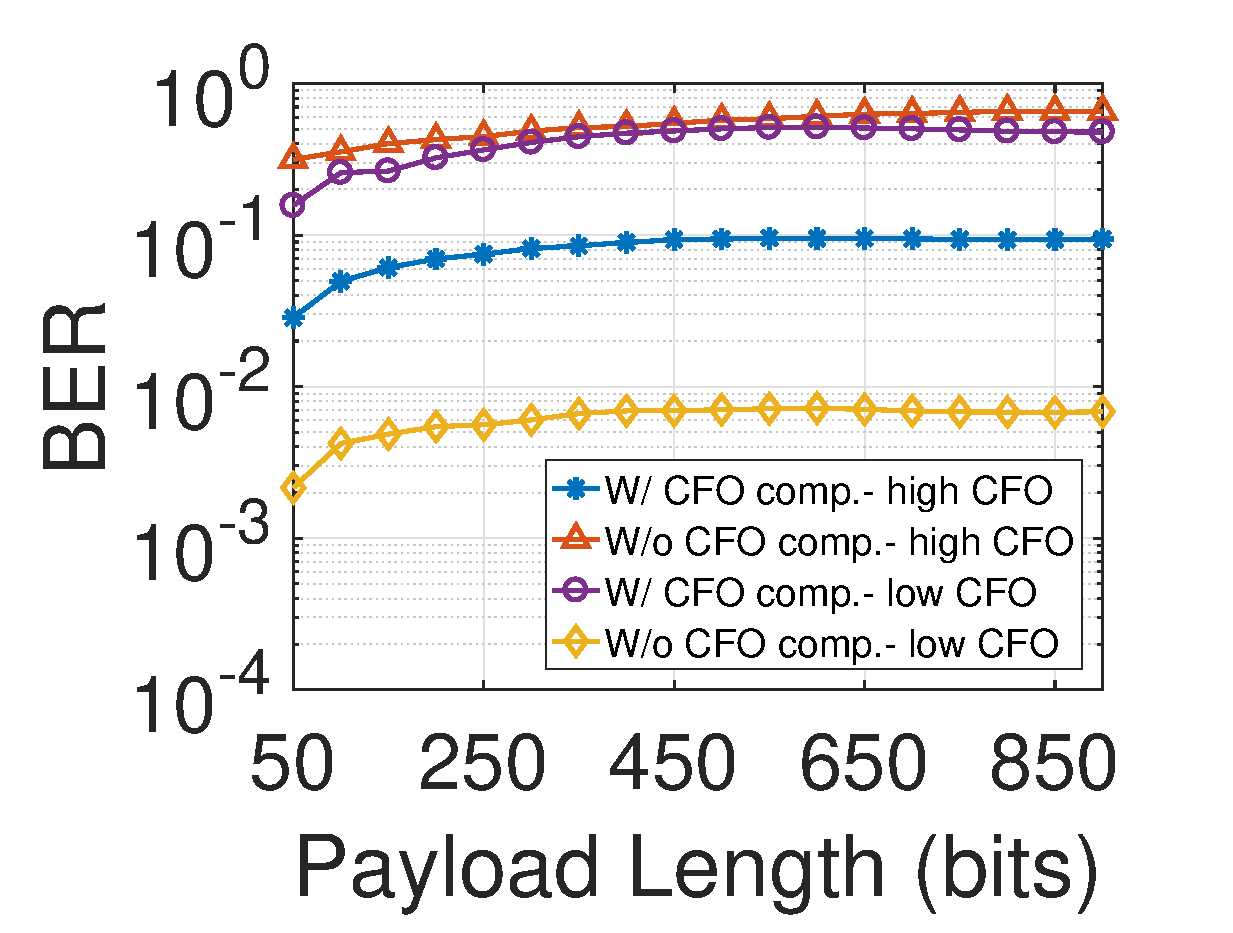
\includegraphics[width=0.47\textwidth]{figures/cfo2} &
     \includegraphics[width=0.47\textwidth]{figures/locations2_new}\\
     (a) CFO compensation & (b) Channel estimation error
     \end{tabular}
    \caption{Effect of CFO and channel estimation error on BER. }
    \label{fig:cfo}
\end{figure}